\documentclass[10pt]{beamer}
\usepackage{../../../resources/themes/algolymp-dense}
\usepackage{booktabs}
\usepackage{amssymb}
\usepackage{tikz}
\usetikzlibrary{matrix, positioning, calc, trees, arrows.meta}

\title{Metoda Backtracking}
\subtitle{Generarea elementelor combinatoriale $\cdot$ Backtracking în plan}
\author{Andrei Mihai Ciobanu}
\institute{Algolymp Summer School}
\date{}
\titlegraphic{\includegraphics[width=3cm]{../../../resources/algolymp-logo.png}}
\setbeamertemplate{frame footer}{Algolymp Summer School}

\begin{document}

\begin{frame}\titlepage\end{frame}

\begin{frame}{Cuprins}\tableofcontents\end{frame}

%% ============================================================
\section{Metoda Backtracking}
%% ============================================================

\begin{frame}{Ce este backtracking?}
  \begin{block}{Definiție}
    \textbf{Backtracking} este o metodă care construiește incremental o soluție,
    luând câte o decizie la fiecare pas \textemdash{} ducând astfel la parcurgerea
    \textbf{tuturor} soluțiilor posibile.
  \end{block}
  \smallskip
  \textbf{Tipuri de probleme:}
  \begin{itemize}\itemsep2pt
    \item \textbf{Enumerare} \textemdash{} generează \textbf{toate} soluțiile (permutări, combinări etc.)
    \item \textbf{Decizie} \textemdash{} există o soluție? (da / nu)
    \item \textbf{Optimizare} \textemdash{} găsește soluția \textbf{cea mai bună}
  \end{itemize}
  \smallskip
  \textbf{Idee centrală:} construim un vector soluție $x[1], x[2], \ldots, x[n]$
  element cu element. La fiecare pas $k$:
  \begin{enumerate}\itemsep1pt
    \item Încercăm pe rând \textbf{toate valorile posibile} pentru $x[k]$
    \item Pentru fiecare valoare: continuăm recursiv la pasul $k+1$
    \item Când terminăm toate valorile: \textbf{revenim} la pasul $k-1$ (\textit{backtrack})
  \end{enumerate}
  \smallskip
  \textbf{Complexitate:} exponențială \textemdash{} în absența oricărei optimizări.
\end{frame}

\begin{frame}{Arborele de decizie \textemdash{} permutări ale $\{1,2,3\}$}
  Fiecare nod = starea vectorului soluție. Ramura = valoarea aleasă la pasul curent.
  Frunzele verzi = soluții complete.
  \begin{center}
  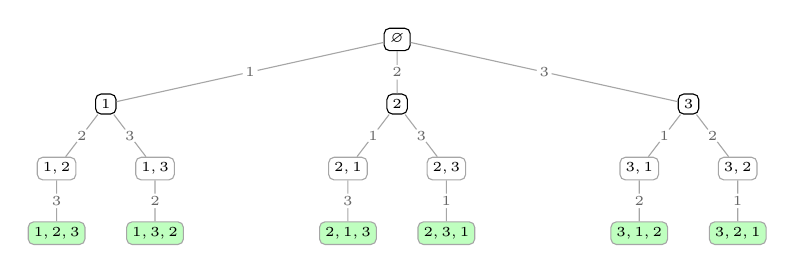
\begin{tikzpicture}[
    level distance=0.82cm,
    level 1/.style={sibling distance=3.7cm},
    level 2/.style={sibling distance=1.25cm},
    every node/.style={draw, rounded corners=2pt, font=\tiny, inner sep=2pt},
    edge from parent/.style={draw, thin, gray!70},
    lbl/.style={draw=none, fill=white, inner sep=1pt, font=\tiny, text=black!60, midway}
  ]
  \node {$\varnothing$}
    child { node {1}
      child { node {1,\,2}
        child { node[fill=green!25] {1,\,2,\,3} edge from parent node[lbl] {3} }
        edge from parent node[lbl] {2}
      }
      child { node {1,\,3}
        child { node[fill=green!25] {1,\,3,\,2} edge from parent node[lbl] {2} }
        edge from parent node[lbl] {3}
      }
      edge from parent node[lbl] {1}
    }
    child { node {2}
      child { node {2,\,1}
        child { node[fill=green!25] {2,\,1,\,3} edge from parent node[lbl] {3} }
        edge from parent node[lbl] {1}
      }
      child { node {2,\,3}
        child { node[fill=green!25] {2,\,3,\,1} edge from parent node[lbl] {1} }
        edge from parent node[lbl] {3}
      }
      edge from parent node[lbl] {2}
    }
    child { node {3}
      child { node {3,\,1}
        child { node[fill=green!25] {3,\,1,\,2} edge from parent node[lbl] {2} }
        edge from parent node[lbl] {1}
      }
      child { node {3,\,2}
        child { node[fill=green!25] {3,\,2,\,1} edge from parent node[lbl] {1} }
        edge from parent node[lbl] {2}
      }
      edge from parent node[lbl] {3}
    };
  \end{tikzpicture}
  \end{center}
  \smallskip
  Arborele se explorează \textbf{în adâncime} (Depth First Seach).
  Pentru $n = 3$: $3! = 6$ frunze = 6 permutări distincte.
\end{frame}

\begin{frame}{Pruning \textemdash{} tăierea ramurilor invalide}
  \begin{block}{Definiție}
    \textbf{Pruning} înseamnă a abandona o ramură a arborelui de decizie
    \textbf{imediat ce} se constată că nu poate duce la o soluție validă \textemdash{} fără
    a mai explora subarborele ei.
  \end{block}
  \smallskip
  \textbf{Exemplu:} secvențe de lungime 2 din $\{1,2,3\}$ cu $x[1] \neq x[2]$.\\
  Nodurile roșii sunt tăiate înainte de a mai continua recursivitatea:
  \begin{center}
  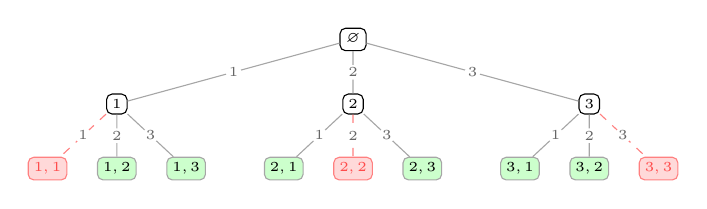
\begin{tikzpicture}[
    level distance=0.82cm,
    level 1/.style={sibling distance=3.0cm},
    level 2/.style={sibling distance=0.88cm},
    every node/.style={draw, rounded corners=2pt, font=\tiny, inner sep=2pt},
    edge from parent/.style={draw, thin, gray!70},
    lbl/.style={draw=none, fill=white, inner sep=1pt, font=\tiny, text=black!60, midway},
    pruned/.style={fill=red!15, draw=red!50, text=red!70}
  ]
  \node {$\varnothing$}
    child { node {1}
      child { node[pruned] {1,\,1} edge from parent[dashed, red!50] node[lbl] {1} }
      child { node[fill=green!20] {1,\,2} edge from parent node[lbl] {2} }
      child { node[fill=green!20] {1,\,3} edge from parent node[lbl] {3} }
      edge from parent node[lbl] {1}
    }
    child { node {2}
      child { node[fill=green!20] {2,\,1} edge from parent node[lbl] {1} }
      child { node[pruned] {2,\,2} edge from parent[dashed, red!50] node[lbl] {2} }
      child { node[fill=green!20] {2,\,3} edge from parent node[lbl] {3} }
      edge from parent node[lbl] {2}
    }
    child { node {3}
      child { node[fill=green!20] {3,\,1} edge from parent node[lbl] {1} }
      child { node[fill=green!20] {3,\,2} edge from parent node[lbl] {2} }
      child { node[pruned] {3,\,3} edge from parent[dashed, red!50] node[lbl] {3} }
      edge from parent node[lbl] {3}
    };
  \end{tikzpicture}
  \end{center}
  \smallskip
  Fără pruning: $3^2 = 9$ frunze. Cu pruning: \textbf{6 frunze} (3 ramuri tăiate).
  Cu constrângeri mai stricte (ex.\ N-Regine), reducerea poate fi \textbf{dramatică}.
\end{frame}

\begin{frame}[fragile]{Schelet general}
  \begin{lstlisting}
int x[nmax + 1], n;

bool valid(int k) {
    // conditia specifica problemei
    // (x[k] compatibil cu x[1..k-1]?)
    return true;
}
void back(int k) {
    if (k > n) {           // solutie completa
        // afiseaza x[1..n]
        return;
    }
    for (int v = /* valori_min */; v <= /* valori_max */; v++) {
        x[k] = v;
        if (valid(k)) {
            back(k + 1);
        }
    }
}
// Apel initial: back(1)
  \end{lstlisting}
  \textbf{Domeniul valorilor} și \textbf{condiția de soluție completă} ($k > n$)
  sunt specifice fiecărei probleme. \texttt{valid()} poate fi inline dacă e simplu.
\end{frame}

%% ============================================================
\section{Elemente combinatoriale}
%% ============================================================

\begin{frame}{Factorial și Permutări \textemdash{} teorie}
  \begin{columns}[T]
  \column{0.50\textwidth}
  \begin{block}{Factorial}
    $n! = 1 \cdot 2 \cdot \ldots \cdot n$ \textemdash{} numărul de moduri de a
    aranja $n$ obiecte distincte. Prin convenție: $0! = 1$.
    $$1!=1,\; 2!=2,\; 3!=6,\; 4!=24,\; 5!=120$$
  \end{block}
  \smallskip
  \begin{block}{Permutări ale $\{1,\ldots,n\}$}
    O \textbf{permutare} este o \textbf{ordonare} a tuturor celor $n$ elemente.
    Număr total:
    $$P(n) = n!$$
  \end{block}
  \column{0.48\textwidth}
  \textbf{Exemplu} ($n = 3$, toate permutările mulțimii $\{1,2,3\}$):
  \smallskip
  \begin{center}
  \begin{tabular}{ccc}
    \toprule
    $x[1]$ & $x[2]$ & $x[3]$ \\
    \midrule
    1 & 2 & 3 \\
    1 & 3 & 2 \\
    2 & 1 & 3 \\
    2 & 3 & 1 \\
    3 & 1 & 2 \\
    3 & 2 & 1 \\
    \bottomrule
  \end{tabular}
  \end{center}
  \smallskip
  Total: $P(3) = 3! = \mathbf{6}$ permutări
  \end{columns}
\end{frame}

\begin{frame}[fragile]{Permutări \textemdash{} implementare}
  \textbf{Cheie:} \texttt{folosit[v]} marchează elementele deja plasate
  $\Rightarrow$ fiecare valoare apare o singură dată.
  \begin{lstlisting}
int x[nmax + 1];
bool folosit[nmax + 1];
int n;

void back(int k) {
    if (k > n) {
        for (int i = 1; i <= n; i++) cout << x[i] << " ";
        cout << "\n";
        return;
    }
    for (int v = 1; v <= n; v++) {
        if (!folosit[v]) {
            x[k] = v;
            folosit[v] = true;
            back(k + 1);
            folosit[v] = false;
        }
    }
}
// Apel: back(1)
  \end{lstlisting}
\end{frame}

\begin{frame}{Aranjamente \textemdash{} teorie}
  \begin{columns}[T]
  \column{0.50\textwidth}
  \begin{block}{Definiție}
    Un \textbf{aranjament} de $p$ elemente din $n$ ($p \leq n$) este o selecție
    \textbf{ordonată} de $p$ elemente \textbf{distincte} din $\{1,\ldots,n\}$.
    $$A(n,p) = \frac{n!}{(n-p)!} = n \cdot (n{-}1) \cdots (n{-}p{+}1)$$
  \end{block}
  \smallskip
  \textbf{Diferența față de permutări:} alegi doar $p < n$ elemente, dar
  \textbf{ordinea contează}: $(1,2) \neq (2,1)$.
  \column{0.48\textwidth}
  \textbf{Exemplu} ($n=4$, $p=2$, din $\{1,2,3,4\}$):
  \begin{itemize}\itemsep0pt
    \item[] $(1,2),\;(1,3),\;(1,4)$
    \item[] $(2,1),\;(2,3),\;(2,4)$
    \item[] $(3,1),\;(3,2),\;(3,4)$
    \item[] $(4,1),\;(4,2),\;(4,3)$
  \end{itemize}
  \smallskip
  Total: $A(4,2) = 4 \cdot 3 = \dfrac{4!}{2!} = \mathbf{12}$ aranjamente
  \end{columns}
\end{frame}

\begin{frame}[fragile]{Aranjamente \textemdash{} implementare}
  \textbf{Identic cu permutările} \textemdash{} singura diferență: oprire la $k > p$
  (am ales $p$ elemente) în loc de $k > n$.
  \begin{lstlisting}
int x[nmax + 1];
bool folosit[nmax + 1];
int n, p;

void back(int k) {
    if (k > p) {       // am ales p elemente
        for (int i = 1; i <= p; i++) cout << x[i] << " ";
        cout << "\n";
        return;
    }
    for (int v = 1; v <= n; v++) {
        if (!folosit[v]) {
            x[k] = v;
            folosit[v] = true;
            back(k + 1);
            folosit[v] = false;
        }
    }
}
// Apel: back(1)
  \end{lstlisting}
\end{frame}

\begin{frame}{Combinări \textemdash{} teorie}
  \begin{columns}[T]
  \column{0.50\textwidth}
  \begin{block}{Definiție}
    O \textbf{combinare} de $p$ elemente din $n$ este o selecție
    \textbf{neordonată} de $p$ elemente distincte din $\{1,\ldots,n\}$.
    $$C(n,p) = \binom{n}{p} = \frac{n!}{p!\,(n-p)!} = \frac{A(n,p)}{p!}$$
  \end{block}
  \smallskip
  \textbf{Diferența față de aranjamente:} ordinea \textbf{nu} contează.\\
  $\{1,2\}$ și $\{2,1\}$ sunt \textbf{aceeași} combinare.\\[4pt]
  Fiecare combinare corespunde la $p!$ aranjamente $\Rightarrow$ împărțim la $p!$.
  \column{0.48\textwidth}
  \textbf{Exemplu} ($n=4$, $p=2$, din $\{1,2,3,4\}$):
  \begin{itemize}\itemsep1pt
    \item[] $\{1,2\},\;\{1,3\},\;\{1,4\}$
    \item[] $\{2,3\},\;\{2,4\}$
    \item[] $\{3,4\}$
  \end{itemize}
  \smallskip
  Total: $C(4,2) = \dfrac{4!}{2!\cdot 2!} = \mathbf{6}$ combinări\\[6pt]
  \textbf{Obs:} $C(4,2) = \dfrac{A(4,2)}{2!} = \dfrac{12}{2} = 6$ \checkmark
  \end{columns}
\end{frame}

\begin{frame}[fragile]{Combinări \textemdash{} implementare}
  \textbf{Cheie:} \texttt{start = x[k-1] + 1} forțează ordine strict crescătoare
  $\Rightarrow$ fără permutări duplicate. Limita \texttt{n - p + k} evită porniri imposibile.
  \begin{lstlisting}
const int nmax = 10;
int x[nmax + 1];
int n, p;

void back(int k) {
    if (k > p) {
        for (int i = 1; i <= p; i++) {
            cout << x[i] << " ";
        }
        cout << "\n";
        return;
    }
    int start = (k == 1) ? 1 : x[k - 1] + 1;
    for (int v = start; v <= n - p + k; v++) {
        x[k] = v;
        back(k + 1);
    }
}
// Apel: back(1)
  \end{lstlisting}
\end{frame}

\begin{frame}{Submulțimi \textemdash{} teorie}
  \begin{columns}[T]
  \column{0.50\textwidth}
  \begin{block}{Definiție}
    O \textbf{submulțime} a lui $\{1,\ldots,n\}$ este orice selecție de
    elemente (inclusiv mulțimea vidă $\varnothing$ și întreaga mulțime).
    $$2^n \text{ submulțimi în total}$$
  \end{block}
  \smallskip
  \textbf{De ce $2^n$?} Fiecare din cele $n$ elemente poate fi
  \textbf{inclus sau exclus} independent:
  $$\underbrace{2 \times 2 \times \cdots \times 2}_{n \text{ elemente}} = 2^n$$
  Spre deosebire de combinări, nu e fixat numărul de elemente alese.
  \column{0.48\textwidth}
  \textbf{Exemplu} ($n=3$, mulțimea $\{1,2,3\}$):
  \smallskip
  \begin{center}
  \begin{tabular}{cl}
    \toprule
    Mască & Submulțime \\
    \midrule
    \texttt{000} & $\varnothing$ \\
    \texttt{001} & $\{1\}$ \\
    \texttt{010} & $\{2\}$ \\
    \texttt{011} & $\{1,2\}$ \\
    \texttt{100} & $\{3\}$ \\
    \texttt{101} & $\{1,3\}$ \\
    \texttt{110} & $\{2,3\}$ \\
    \texttt{111} & $\{1,2,3\}$ \\
    \bottomrule
  \end{tabular}
  \end{center}
  Total: $2^3 = \mathbf{8}$ submulțimi
  \end{columns}
\end{frame}

\begin{frame}[fragile]{Submulțimi \textemdash{} BT: alegere element următor}
  \begin{columns}[T]
  \column{0.50\textwidth}
  Afișăm submulțimea curentă la fiecare apel, apoi \textbf{extindem} cu elemente
  mai mari decât ultimul ales.
  \begin{lstlisting}
int x[nmax + 1], len, n;

void back(int last) {
    for (int i = 1; i <= len; i++) cout << x[i] << " ";
    cout << "\n";
    for (int v = last + 1; v <= n; v++) {
        x[++len] = v;
        back(v);
        len--;
    }
}
// Apel: back(0)
  \end{lstlisting}
  $2^n$ apeluri \textemdash{} câte unul per submulțime.
  \column{0.48\textwidth}
  \centering
  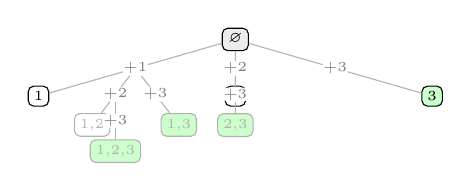
\begin{tikzpicture}[
    level distance=0.72cm,
    level 1/.style={sibling distance=2.5cm},
    level 2/.style={sibling distance=1.1cm},
    level 3/.style={sibling distance=0.65cm},
    every node/.style={draw,rounded corners=2pt,font=\tiny,inner sep=2pt},
    edge from parent/.style={draw,thin,gray!60},
    lbl/.style={draw=none,fill=white,inner sep=0.5pt,font=\tiny,text=black!50,midway}
  ]
  \node[fill=gray!15] {$\varnothing$}
    child { node {1} edge from parent node[lbl]{$+1$}
      child { node {1,2} edge from parent node[lbl]{$+2$}
        child { node[fill=green!20] {1,2,3} edge from parent node[lbl]{$+3$} }
      }
      child { node[fill=green!20] {1,3} edge from parent node[lbl]{$+3$} }
    }
    child { node {2} edge from parent node[lbl]{$+2$}
      child { node[fill=green!20] {2,3} edge from parent node[lbl]{$+3$} }
    }
    child { node[fill=green!20] {3} edge from parent node[lbl]{$+3$} };
  \end{tikzpicture}
  \end{columns}
\end{frame}

\begin{frame}[fragile]{Submulțimi \textemdash{} BT: include/exclude}
  \begin{columns}[T]
  \column{0.50\textwidth}
  La fiecare pas decidem dacă \textbf{includem sau nu} elementul $i$.
  \begin{lstlisting}
int x[nmax + 1], len, n;

void back(int i) {
    if (i > n) {
        for (int j = 1; j <= len; j++) cout << x[j] << " "; cout << "\n"; return;
    }
    back(i + 1);          // nu luam
    x[++len] = i; back(i + 1); len--;  // luam
}
// Apel: back(1)
  \end{lstlisting}
  \column{0.48\textwidth}
  \centering
  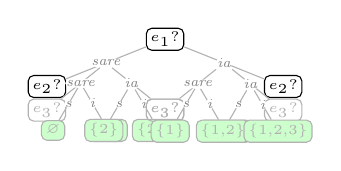
\begin{tikzpicture}[
    level distance=0.60cm,
    level 1/.style={sibling distance=3.0cm},
    level 2/.style={sibling distance=1.5cm},
    level 3/.style={sibling distance=0.70cm},
    every node/.style={draw,rounded corners=2pt,font=\tiny,inner sep=1.5pt},
    edge from parent/.style={draw,thin,gray!60},
    lbl/.style={draw=none,fill=white,inner sep=0.5pt,font=\tiny\itshape,text=black!50,midway}
  ]
  \node {$e_1$?}
    child { node {$e_2$?} edge from parent node[lbl]{sare}
      child { node {$e_3$?} edge from parent node[lbl]{sare}
        child { node[fill=green!20] {$\varnothing$} edge from parent node[lbl]{s} }
        child { node[fill=green!20] {\{3\}} edge from parent node[lbl]{i} }
      }
      child { node {$e_3$?} edge from parent node[lbl]{ia}
        child { node[fill=green!20] {\{2\}} edge from parent node[lbl]{s} }
        child { node[fill=green!20] {\{2,3\}} edge from parent node[lbl]{i} }
      }
    }
    child { node {$e_2$?} edge from parent node[lbl]{ia}
      child { node {$e_3$?} edge from parent node[lbl]{sare}
        child { node[fill=green!20] {\{1\}} edge from parent node[lbl]{s} }
        child { node[fill=green!20] {\{1,3\}} edge from parent node[lbl]{i} }
      }
      child { node {$e_3$?} edge from parent node[lbl]{ia}
        child { node[fill=green!20] {\{1,2\}} edge from parent node[lbl]{s} }
        child { node[fill=green!20] {\{1,2,3\}} edge from parent node[lbl]{i} }
      }
    };
  \end{tikzpicture}
  \end{columns}
  \smallskip
  \textbf{Obs:} $2^{n+1}{-}1$ apeluri vs.\ $2^n$ \textemdash{} nodurile interne nu afișează nimic
  (decizii goale). La alegerea elementului următor \textbf{fiecare apel = o submulțime afișată}.
\end{frame}

\begin{frame}[fragile]{Submulțimi \textemdash{} implementare (măști de biți)}
  Fiecare întreg $\texttt{mask} \in [0, 2^n)$ codifică o submulțime:
  bitul $i$ = 1 înseamnă că elementul $i+1$ este inclus.
  \begin{lstlisting}
int a[nmax + 1], n;

for (int mask = 0; mask < (1 << n); mask++) {
    for (int i = 0; i < n; i++) {
        if (mask & (1 << i)) {
            cout << a[i + 1] << " ";
        }
    }
    cout << "\n";
}
  \end{lstlisting}
  Eficient pentru $n \leq 20$ \textemdash{} $2^{20} \approx 10^6$ iterații.
  \smallskip
  \textbf{Bonus \textemdash{} combinări cu bitmask:} selectăm doar măștile cu exact
  $p$ biți setați (folosind \texttt{\_\_builtin\_popcount(mask) == p}).
  Mai ineficient decât BT clasic, dar util când avem deja bitmask-ul submulțimii.
\end{frame}

\begin{frame}{Produs cartezian \textemdash{} teorie}
  \begin{columns}[T]
  \column{0.50\textwidth}
  \begin{block}{Definiție}
    Produsul cartezian $A_1 \times A_2 \times \cdots \times A_n$ este mulțimea
    tuturor secvențelor $(x_1, \ldots, x_n)$ cu $x_k \in A_k$ pentru fiecare $k$.
    $$|A_1 \times \cdots \times A_n| = \prod_{k=1}^{n} |A_k|$$
  \end{block}
  \smallskip
  \textbf{Diferența față de permutări:} valorile nu trebuie să fie distincte;
  fiecare poziție are \textbf{propriul domeniu} de valori.\\[4pt]
  Dacă $|A_k| = m$ pentru orice $k$: total $m^n$ secvențe.
  \column{0.48\textwidth}
  \textbf{Exemplu:} $A_1 = \{1,2\}$, $A_2 = \{1,2,3\}$\\[4pt]
  Toate perechile $(x_1, x_2)$:
  \begin{center}
  \begin{tabular}{cc}
    \toprule
    $x_1$ & $x_2$ \\
    \midrule
    1 & 1 \\
    1 & 2 \\
    1 & 3 \\
    2 & 1 \\
    2 & 2 \\
    2 & 3 \\
    \bottomrule
  \end{tabular}
  \end{center}
  Total: $2 \times 3 = \mathbf{6}$ secvențe\\
  \small(obs: $(1,1)$ și $(2,2)$ sunt valide \textemdash{} repetiții permise!)
  \end{columns}
\end{frame}

\begin{frame}[fragile]{Produs cartezian \textemdash{} implementare}
  \textbf{Cheie:} fără \texttt{folosit[]} \textemdash{} fiecare poziție $k$ parcurge
  independent valorile $1 \ldots \texttt{lim}[k]$ (repetiții permise).
  \begin{lstlisting}
const int nmax = 10;
int x[nmax + 1];
int lim[nmax + 1];
int n;

void back(int k) {
    if (k > n) {
        for (int i = 1; i <= n; i++) {
            cout << x[i] << " ";
        }
        cout << "\n";
        return;
    }
    for (int v = 1; v <= lim[k]; v++) {
        x[k] = v;
        back(k + 1);
    }
}
// Apel: back(1)
  \end{lstlisting}
\end{frame}

%% ============================================================
\section{Backtracking în plan}
%% ============================================================

\begin{frame}{Problema N Reginelor \textemdash{} formulare}
  \begin{columns}[T]
  \column{0.55\textwidth}
  \begin{block}{Problemă}
    Plasează $n$ regine pe o tablă de șah $n \times n$ astfel încât
    nicio două regine să nu se atace reciproc (pe linie, coloană sau diagonală).
  \end{block}
  \smallskip
  \textbf{Modelare:} $x[i]$ = coloana reginei de pe rândul $i$.
  Deoarece punem exact o regină per rând, conflictele pe linie sunt
  excluse automat. Rămân de verificat:
  \begin{itemize}\itemsep2pt
    \item \textbf{Coloană:} $x[i] \neq x[j]$ pentru $i \neq j$
    \item \textbf{Diagonală:} $|x[i]-x[j]| \neq |i-j|$ pentru $i \neq j$
  \end{itemize}
  \smallskip
  \textbf{Complexitate:} exponențială, dar pruning-ul reducesemnificativ
  spațiul de căutare. Pentru $n = 8$: \textbf{92 soluții}.
  \column{0.43\textwidth}
  \begin{center}
  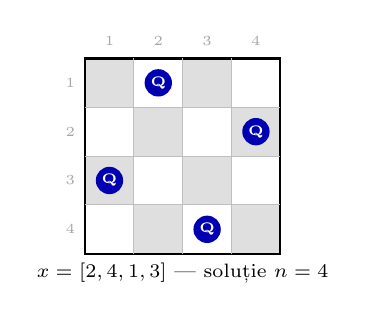
\begin{tikzpicture}[scale=0.62]
    % Tabla 4x4, solutia [2,4,1,3]
    \foreach \r/\c in {1/1, 1/3, 2/2, 2/4, 3/1, 3/3, 4/2, 4/4} {
      \fill[gray!25] (\c-1, 4-\r) rectangle ++(1,1);
    }
    \draw[thick] (0,0) rectangle (4,4);
    \foreach \i in {1,2,3} {
      \draw[gray!50] (\i,0) -- (\i,4);
      \draw[gray!50] (0,\i) -- (4,\i);
    }
    % Regine la [2,4,1,3]
    \foreach \r/\c in {1/2, 2/4, 3/1, 4/3} {
      \fill[blue!70!black] (\c-0.5, 4.5-\r) circle (0.28);
      \node[font=\tiny\bfseries, text=white] at (\c-0.5, 4.5-\r) {Q};
    }
    % Etichete rand
    \foreach \i in {1,...,4} {
      \node[font=\tiny, text=gray!70] at (-0.3, 4.5-\i) {\i};
    }
    % Etichete coloana
    \foreach \i in {1,...,4} {
      \node[font=\tiny, text=gray!70] at (\i-0.5, 4.35) {\i};
    }
    % x[] label
    \node[font=\scriptsize] at (2, -0.4) {$x = [2, 4, 1, 3]$ \textemdash{} soluție $n=4$};
  \end{tikzpicture}
  \end{center}
  \end{columns}
\end{frame}

\begin{frame}[fragile]{N Regine \textemdash{} valid()}
  Verificăm noua regină față de toate cele plasate anterior pe rândurile $1 \ldots k{-}1$.
  \begin{lstlisting}
const int nmax = 20;
int x[nmax + 1];
int n;

bool valid(int k) {
    for (int i = 1; i < k; i++) {
        if (x[i] == x[k]) {
            return false;  // aceeasi coloana
        }
        if (abs(x[i] - x[k]) == abs(i - k)) {
            return false;  // aceeasi diagonala
        }
    }
    return true;
}
  \end{lstlisting}
  \textbf{Optimizare $O(1)$:} în loc de bucla din \texttt{valid()}, menține tablouri
  \texttt{col[c]}, \texttt{diag1[r-c+n]}, \texttt{diag2[r+c]} marcând
  coloanele/diagonalele ocupate.
\end{frame}

\begin{frame}[fragile]{N Regine \textemdash{} back()}
  \begin{lstlisting}
void back(int k) {
    if (k > n) {
        for (int i = 1; i <= n; i++) { cout << x[i] << " "; }
        cout << "\n";
        return;
    }
    for (int col = 1; col <= n; col++) {
        x[k] = col;
        if (valid(k)) {
            back(k + 1);
        }
    }
}
// Apel: back(1)
  \end{lstlisting}
  \textbf{Pruning:} \texttt{valid()} taie ramura imediat \textemdash{} pentru $n=8$
  se vizitează doar $\sim$15000 noduri din $8^8 \approx 16 \times 10^6$ posibile.
  Total \textbf{92 soluții} pentru $n=8$.
\end{frame}

\begin{frame}{Traseul Calului (\textit{Knight's Tour})}
  \begin{columns}[T]
  \column{0.52\textwidth}
  \begin{block}{Problemă}
    Plasează un cal de șah pe o tablă $n \times n$ astfel încât să
    viziteze fiecare celulă \textbf{exact o dată} (lanț hamiltonian).
  \end{block}
  \smallskip
  Calul se mișcă în L: $(\pm 1, \pm 2)$ sau $(\pm 2, \pm 1)$ \textemdash{} 8
  mișcări posibile per celulă.
  \smallskip
  \begin{block}{Algoritmul Warnsdorff (1823) \textemdash{} o euristică}
    Alege la fiecare pas mișcarea care duce în celula cu
    \textbf{cele mai puține ieșiri nevizitate}.\\[2pt]
    BT pur: $O(8^{n^2})$. Cu Warnsdorff: $O(n^2)$ în practică.
  \end{block}
  \column{0.46\textwidth}
  \begin{center}
    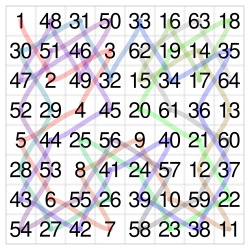
\includegraphics[width=\linewidth]{knight_tour.png}
    \par{\scriptsize Traseu complet pe tablă $8\times 8$ (numerele indică ordinea mișcărilor)}
  \end{center}
  \end{columns}
\end{frame}

\begin{frame}[fragile]{Traseul Calului \textemdash{} implementare BT}
  \begin{lstlisting}
const int nmax = 8;
int tabla[nmax + 1][nmax + 1];
int dx[] = {-2,-2,-1,-1, 1, 1, 2, 2};
int dy[] = {-1, 1,-2, 2,-2, 2,-1, 1};
int n;
bool valid(int x, int y) {
    return x >= 1 && x <= n && y >= 1 && y <= n
        && tabla[x][y] == 0;
}
void back(int x, int y, int pas) {
    tabla[x][y] = pas;
    if (pas == n * n) {
        // afiseaza tabla[][]
        tabla[x][y] = 0; return;
    }
    for (int d = 0; d < 8; d++) {
        int nx = x + dx[d], ny = y + dy[d];
        if (valid(nx, ny)) { back(nx, ny, pas + 1); }
    }
    tabla[x][y] = 0;  // backtrack
}
// Apel: back(1, 1, 1)
  \end{lstlisting}
\end{frame}

%% ============================================================
\section{Alte aplicații}
%% ============================================================

\begin{frame}{Backtracking \textemdash{} când e optim și când nu}
  \begin{itemize}\itemsep2pt
    \item \textbf{Permutări / Aranjamente / Combinări / Submulțimi}\\
      \hspace{1em}$\rightarrow$ BT \textbf{optim} (trebuie generate toate soluțiile)

    \item \textbf{N-Regine, Sudoku, Colorarea grafurilor}\\
      \hspace{1em}$\rightarrow$ BT cu pruning \textbf{standard}; soluție exponențială inevitabilă

    \item \textbf{Rucsac 0/1} \textemdash{} DP $O(nW)$ când $W$ mic;
      \alert{BT + Branch\,\&\,Bound} când $W$ enorm (100p, $\leq 1\,$ms/test)

    \item \textbf{Problema spectacolelor}\\
      \hspace{1em}BT: $O(2^n)$ \hfill \alert{mai bine: Greedy $O(n \log n)$}

    \item \textbf{Traseul Calului} \textemdash{} BT pur: exponențial
      \hfill \alert{mai bine: Warnsdorff $O(n^2)$}

    \item \textbf{Lanț / ciclu hamiltonian, SAT, Colorare optimală}\\
      \hspace{1em}$\rightarrow$ Probleme \textbf{NP-complete}: BT e abordarea clasică
  \end{itemize}
  \textbf{Regulă practică:} dacă $n \leq 20$\textendash{}25, BT e viabil.
  Dacă $n$ e mare, caută structură exploatabilă (DP, Greedy, B\&B \ldots).
\end{frame}

\begin{frame}{Rucsac 0/1 \textemdash{} Branch \& Bound}
  \begin{columns}[T]
  \column{0.50\textwidth}
  \begin{block}{Problema}
    $n$ obiecte cu greutăți $w_i$, profituri $p_i$, rucsac de capacitate $W$.
    Maximizăm profitul fără a depăși $W$.
  \end{block}
  \textbf{De ce nu DP?} $O(nW)$ \textemdash{} imposibil la $W \leq 10^9$.\\
  BT + B\&B: 100p pe infoarena, $\leq 1\,$ms/test.
  \column{0.48\textwidth}
  \textbf{Cele 4 optimizări:}
  \begin{enumerate}\itemsep2pt
    \item \textbf{Sortare} după $p_i/w_i$ descrescător
    \item \textbf{Bound optimist:} rucsac fracționar ca upper bound
    \item \textbf{Init greedy:} $\mathit{max\_profit}$ bun $\Rightarrow$ pruning agresiv
    \item \textbf{Take first:} luăm înainte de a renunța la obiect
  \end{enumerate}
  \smallskip
  Dacă $\mathit{profit} + \mathit{bestSuffix}(i, W{-}\mathit{weight}) \leq \mathit{max\_profit}$:\\
  \hspace{1em}$\rightarrow$ tăiem ramura (pruning).
  \end{columns}
\end{frame}

\begin{frame}[fragile]{Rucsac 0/1 \textemdash{} implementare B\&B}
  \begin{lstlisting}
// a[i] = {w, p}, sortat dupa p/w desc; max_profit initializat greedy
long long weight = 0, profit = 0, max_profit;
long double bestSuffix(int i, long long rem) {
    long double best = 0;
    for (int j = i; j <= n && rem > 0; ++j) {
        long long aux = min(rem, a[j].first);
        best += 1.0L * a[j].second * aux / a[j].first;
        rem -= aux;
    }
    return best;
}
void backtrack(int i) {
    if (i > n) { max_profit = max(max_profit, profit); return; }
    if (profit + bestSuffix(i, W - weight) <= max_profit) return;
    weight += a[i].first; profit += a[i].second;
    if (weight <= W) backtrack(i + 1);
    weight -= a[i].first; profit -= a[i].second;
    backtrack(i + 1);
}
  \end{lstlisting}
\end{frame}

\begin{frame}{\texttt{next\_permutation} \textemdash{} generare fără recursivitate}
  \begin{columns}[T]
  \column{0.52\textwidth}
  \textbf{Idee:} pentru permutarea curentă, găsim \textit{succesoarea} în ordine
  lexicografică, repetând până epuizăm toate $n!$ permutări.
  \begin{block}{Algoritmul (3 pași)}
    \begin{enumerate}\itemsep1pt
      \item Găsim cel mai din dreapta $i$ cu $x[i] < x[i+1]$\\ (prefixul descrescător de la final)
      \item Găsim cel mai mic $x[j] > x[i]$ cu $j > i$\\ și îl schimbăm cu $x[i]$
      \item Inversăm sufixul $x[i+1\,.\,.\,n]$
    \end{enumerate}
  \end{block}
  \column{0.46\textwidth}
  \textbf{Exemplu} $\{1,3,2\} \rightarrow \{2,1,3\}$:
  \begin{itemize}\itemsep1pt
    \item[] $x[1]{=}1 < x[2]{=}3$ $\Rightarrow$ $i=1$
    \item[] Cel mai mic $x[j]>1$ cu $j>1$: $x[2]{=}2$\\
      {\small (după inversarea sufixului $3,2 \rightarrow 2,3$)}
    \item[] Swap $x[1] \leftrightarrow x[2]$: $\{2,1,3\}$
    \item[] Inversare sufix: $\{2,1,3\}$
  \end{itemize}
  \smallskip
  \textbf{Complexitate:} $O(n)$/permutare; $O(n \cdot n!)$ total.\\
  \alert{Identic ca backtracking, dar fără stivă recursivă.}
  \end{columns}
\end{frame}

\begin{frame}[fragile]{\texttt{next\_permutation} \textemdash{} implementare}
  \begin{lstlisting}
bool nextPermutation(int x[], int n) {
    int i = n - 1;
    while (i > 0 && x[i] >= x[i + 1]) i--;
    if (i == 0) return false; // ultima permutare
    int j = n;
    while (x[j] <= x[i]) j--;
    swap(x[i], x[j]);
    // inversam sufixul x[i+1..n]
    int l = i + 1, r = n;
    while (l < r) { swap(x[l], x[r]); l++; r--; }
    return true;
}

// Generare toate permutarile lui {1..n}:
// initializare: x[i] = i (permutarea 1,2,...,n)
do {
    for (int i = 1; i <= n; i++) cout << x[i] << " ";
    cout << "\n";
} while (nextPermutation(x, n));
// SAU direct: std::next_permutation(x + 1, x + n + 1)
  \end{lstlisting}
\end{frame}

%% ============================================================
\section{Recapitulare}
%% ============================================================

\begin{frame}{Termeni importanți}
  \begin{itemize}\itemsep5pt
    \item \textbf{Backtracking} \textemdash{} metodă de construire incrementală a
      unei soluții prin explorarea \textbf{tuturor} posibilităților (DFS în
      arborele de decizie). La fiecare pas încearcă toate valorile, după care
      \textbf{revine} (\textit{backtrack}) la pasul anterior.

    \item \textbf{Arbore de decizie} \textemdash{} structură în care fiecare nod
      reprezintă o stare parțială a soluției, fiecare ramură o decizie, iar
      frunzele soluțiile complete (sau ramuri tăiate).

    \item \textbf{Pruning} (tăierea ramurilor) \textemdash{} abandonarea unui subarbore
      \textbf{imediat ce} se constată că nu poate duce la o soluție validă, fără
      a-l mai explora. Reduce exponențial spațiul de căutare la probleme cu
      constrângeri stricte (ex.\ N-Regine, Sudoku).

    \item \textbf{Euristică} \textemdash{} regulă de decizie \textbf{aproximativă}
      care ghidează căutarea spre soluții bune fără a garanta optimalul.
      Exemplu: algoritmul Warnsdorff pentru traseul calului (alege celula cu
      cele mai puține ieșiri libere) \textemdash{} funcționează excelent în
      practică, dar nu e demonstrat matematic pentru orice $n$.
  \end{itemize}
\end{frame}

\begin{frame}{Probleme educaționale}
  \begin{enumerate}\footnotesize\itemsep1pt
    \item \href{https://code.algolymp.com/problems/1704}{\textbf{All Permutations of 1 to N}}
          \textcolor{gray}{(AlgoCode \#1704)}
    \item \href{https://code.algolymp.com/problems/1705}{\textbf{Cartesian Product Generation}}
          \textcolor{gray}{(AlgoCode \#1705)}
    \item \href{https://code.algolymp.com/problems/1364}{\textbf{N Queens Board}}
          \textcolor{gray}{(AlgoCode \#1364)}
    \item \href{https://code.algolymp.com/problems/1373}{\textbf{Arrangements of k Elements}}
          \textcolor{gray}{(AlgoCode \#1373)}
    \item \href{https://code.algolymp.com/problems/1374}{\textbf{Subsets of k Elements}}
          \textcolor{gray}{(AlgoCode \#1374)}
    \item \href{https://code.algolymp.com/problems/1375}{\textbf{Nonempty Subsets}}
          \textcolor{gray}{(AlgoCode \#1375)}
    \item \href{https://code.algolymp.com/problems/1376}{\textbf{Distinct Word Anagrams}}
          \textcolor{gray}{(AlgoCode \#1376)}
    \item \href{https://code.algolymp.com/problems/1412}{\textbf{Balanced Bracket Strings}}
          \textcolor{gray}{(AlgoCode \#1412)}
  \end{enumerate}
\end{frame}

\begin{frame}{Probleme de antrenament}
  \begin{enumerate}\footnotesize\itemsep0pt
    \item \href{https://code.algolymp.com/problems/1379}{\textbf{Anagrams with Fixed Vowels}}
          \textcolor{gray}{(AlgoCode \#1379)}
    \item \href{https://code.algolymp.com/problems/1383}{\textbf{Binary Sequences with Same Digit Counts}}
          \textcolor{gray}{(AlgoCode \#1383)}
    \item \href{https://code.algolymp.com/problems/1386}{\textbf{Constrained Digit Generation}}
          \textcolor{gray}{(AlgoCode \#1386)}
    \item \href{https://code.algolymp.com/problems/1403}{\textbf{Increasing Sum Decompositions}}
          \textcolor{gray}{(AlgoCode \#1403)}
    \item \href{https://code.algolymp.com/problems/1404}{\textbf{Signed Squares Equal N}}
          \textcolor{gray}{(AlgoCode \#1404)}
    \item \href{https://code.algolymp.com/problems/1405}{\textbf{Bounded Banknote Payment}}
          \textcolor{gray}{(AlgoCode \#1405)}
    \item \href{https://code.algolymp.com/problems/1406}{\textbf{Cube Towers}}
          \textcolor{gray}{(AlgoCode \#1406)}
    \item \href{https://code.algolymp.com/problems/1411}{\textbf{Distinct Sum Decompositions}}
          \textcolor{gray}{(AlgoCode \#1411)}
    \item \href{https://code.algolymp.com/problems/1414}{\textbf{Fazan Word Chains}}
          \textcolor{gray}{(AlgoCode \#1414)}
    \item \href{https://code.algolymp.com/problems/1703}{\textbf{Permutations with Min and Max Fixed}}
          \textcolor{gray}{(AlgoCode \#1703)}
    \item \href{https://code.algolymp.com/problems/4395}{\textbf{Blocked Queens}}
          \textcolor{gray}{(AlgoCode \#4395)}
    \item \href{https://code.algolymp.com/problems/1370}{\textbf{Digit Difference Numbers}}
          \textcolor{gray}{(AlgoCode \#1370)}
    \item \href{https://code.algolymp.com/problems/1706}{\textbf{Special Increasing Sequences}}
          \textcolor{gray}{(AlgoCode \#1706)}
    \item \href{https://code.algolymp.com/problems/1707}{\textbf{Reciprocal Sum Sequences}}
          \textcolor{gray}{(AlgoCode \#1707)}
  \end{enumerate}
\end{frame}

\begin{frame}{Resurse}
  \begin{itemize}\itemsep4pt
    \item \textbf{pbinfo.ro} \textemdash{} Capitolul ``Metoda Backtracking''\\
      Teorie + pseudocod + probleme clasice (permutări, regine, labirint)

    \item \textbf{pbinfo.ro} \textemdash{} ``Generarea permutărilor / aranjamentelor /
      combinărilor / submulțimilor''\\
      Cod complet pentru fiecare tip de generare

    \item \textbf{GeeksforGeeks} \textemdash{} ``Introduction to Backtracking''\\
      Arbore de stări, pruning, N-Queens, Sudoku cu explicații vizuale

    \item \textbf{HackerEarth} \textemdash{} ``Recursion and Backtracking''\\
      Recursivitate ca mecanism, backtracking ca strategie, exemplu labirint

    \item \textbf{Wikipedia} \textemdash{} ``Eight queens puzzle''\\
      92 soluții pentru $n=8$, variante, complexitate

    \item \textbf{Wikipedia} \textemdash{} ``Knight's tour''\\
      Algoritmul Warnsdorff, pătrate magice cu traseu de cal
  \end{itemize}
\end{frame}

\end{document}
